\documentclass[portuguese,12pt,a4paper]{article}
\usepackage[T1]{fontenc}
\usepackage{graphicx}
\usepackage{mathtools}
\usepackage{amssymb}
\usepackage{amsthm}
\usepackage{thmtools}
\usepackage{xcolor}
\usepackage{nameref}
\usepackage{babel}
\usepackage{authblk}
\usepackage{fourier}
\usepackage{indentfirst}
\usepackage{float}
\usepackage[colorlinks, urlcolor=blue]{hyperref}
\title{Introdução à Neurociência Computacional\\Lista de Exercícios 1}
\author{Paulo R. Sturion}
\begin{document}
	\maketitle
	
	\noindent Todos os códigos escritos para produzir os resultados dos exercícios a seguir estão disponibilizados de forma clara e organizada no repositório Github: 
	
	\begin{center}
	\noindent \href{https://github.com/prsturion/intro-computational-neurosciene.git}{https://github.com/prsturion/intro-computational-neurosciene.git} \newline
	\end{center}

	\noindent\textbf{Questão 1.} Considere que na equação da membrana (deduzida na aula 4) a corrente injetada 
	$I$ é descrita em termos da densidade de corrente $J$ como 
	$I = JA,$
	onde $A$ é a área da superfície da membrana da célula em cm$^2$. 
	Rescreva a equação da membrana em termos da condutância e da capacitância específicas, $g_m$ e $C_m$, 
	e da densidade de corrente $J$, de maneira que o termo $dV/dt$ esteja isolado no lado esquerdo da equação 
	e todos os outros termos estejam do lado direito. Suponha que as unidades de $g_m$ sejam $[\mu S/cm^2]$, as de $C_m$ sejam $[\mu F/cm^2]$, 
	as de $J$ sejam $[\mu A/cm^2]$ e que as unidades de $V$ e $t$ sejam $[mV]$ e $[ms]$, respectivamente. 
	Preste atenção para que todas as suas unidades sejam: milivolts, milissegundos e microamperes/microsiemens/microfarads 
	por centímetro quadrado.
	\\\\
	
	\noindent\textbf{Resposta:} Reescrevendo a equação de membrana:
	
	\begin{align*}
		\tau \frac{dV_m(t)}{dt} &= -V_m(t) + E + R I_{\text{inj}} \\
		C \frac{dV_m(t)}{dt} &= g(-V_m(t) + E) + I_{\text{inj}} \\
		\frac{C}{A} \frac{dV_m(t)}{dt} &= \frac{g}{A}(-V_m(t) + E) + \frac{I_{\text{inj}}}{A} \\
		C_m \frac{dV_m(t)}{dt} &= g_m(-V_m(t) + E) + J_{\text{inj}} \\
		\frac{dV_m(t)}{dt} &= \frac{1}{C_m}[g_m(E - V_m(t)) + J_{\text{inj}}]
	\end{align*}\\
	
	Para que se possa  utilizar a equação nas unidades requeridas pelo enunciado, deve-se fazer uma correção no primeiro termo por um fator $10^{-3}$.
	
	$$\frac{dV_m(t)}{dt} = \frac{1}{C_m}[g_m(E - V_m(t))10^{-3} + J_{\text{inj}}]$$\\
	
	\noindent \textbf{Questão 2.} Resolva numericamente pelo método de Euler a equação diferencial da questão anterior fazendo $C_m = 1$, $g_m = 100$, $E = 0$ e $V(0) = 0$. Suponha que o estímulo de corrente seja do tipo degrau com $J = 2$ aplicada em $t = 5$ e ``desligada'' em $t = 50$. Utilize $\Delta t = 1$ como passo de tempo. Apresente o resultado da sua solução em um gráfico $V \times t$, com $0 < t < 80$.\\\\
	
	\noindent\textbf{Resposta:} Abaixo está a solução numérica pelo método de Euler para a equação da membrana com os valores do enunciado:
	
	
	
	\begin{figure}[H]
		\centering
		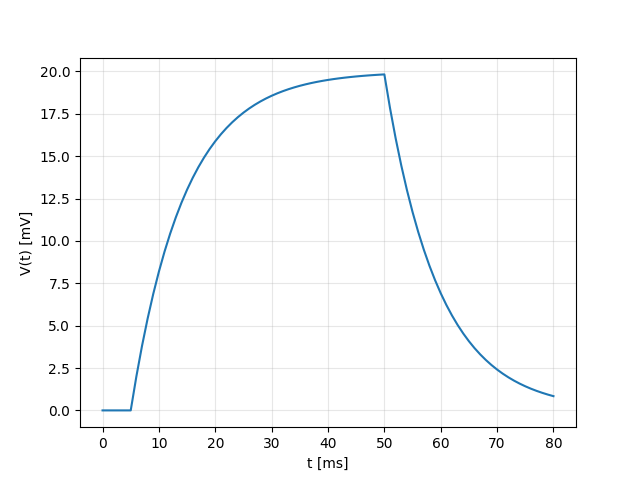
\includegraphics[width=12cm]{../ex_2.png}
		\caption{Solução por método de Euler da equação da membrana para os parâmetros da Questão 2.\\\\}
	\end{figure}
	
	
	\noindent\textbf{Questão 3.} Repita o que foi feito na questão anterior para os seguintes valores de $g_m$: $200$, $100$, $50$, $20$, $10$. Apresente os resultados das suas soluções em um único gráfico $V \times t$ com as curvas superpostas, indicando qual o valor de $g_m$ para cada uma delas. Interprete o resultado mostrado no gráfico.\\\\
	
	\noindent\textbf{Resposta:} Abaixo está a solução gráfica para os diferentes valores de $g_m$.
	
	\begin{figure}[H]
		\centering
		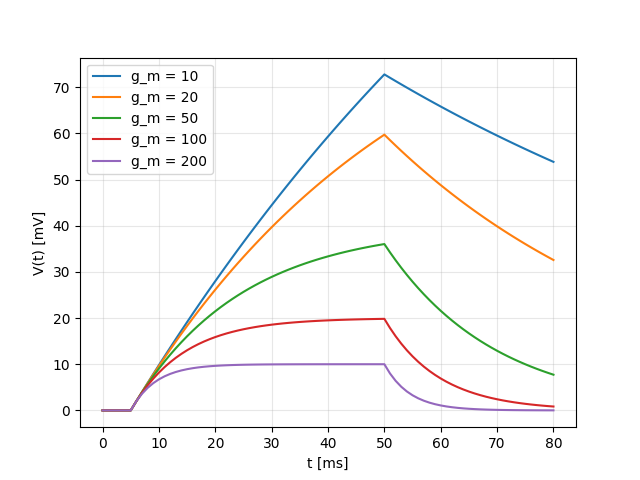
\includegraphics[width=12cm]{../ex_3.png}
		\caption{Solução por método de Euler da equação da membrana para os parâmetros da Questão 3.}
	\end{figure}
	
	O resultado gráfico mostra que quanto maior a condutância, menor é a tensão de equilíbrio, e mais rápido o neurônio a atinge.\\\\
	
	\noindent\textbf{Questão 4.} Na Questão 1, para escrever a equação nas unidades pedidas você teve que multiplicar um dos termos pelo fator $10^{-3}$. Esse tipo de ajuste facilita a ocorrência de erros, pois é fácil esquecer de adicionar o fator multiplicativo quando se implementa a solução numérica. Uma boa prática para resolver numericamente equações diferenciais e evitar o uso de fatores de ajuste de unidades como o usado nas questões acima, adotada por praticamente todos os programas de simulação numérica em neurociência computacional, é converter todas as unidades para o Sistema Internacional (SI) (isto é, escrever as voltagens em volts, os tempos em segundos, as condutâncias em siemens, as capacitâncias em farads, etc). A(s) equação(ões) escrita(s) no SI é(são) resolvida(s) numericamente e depois, para construir os gráficos mostrando os resultados, as unidades das quantidades são convertidas de volta para aquelas mais usuais em neurociência. Reescreva a EDO da Questão 1 com as unidades de todas as quantidades envolvidas no SI. Use os mesmos valores numéricos das quantidades dadas na Questão 2. Em seguida, resolva a EDO pelo método de Euler com $\Delta t = 10^{-3}\,s$ (isto é, 1 ms) e apresente o gráfico de $V \times t$ com $0 < t < 80$.
	\\\\
	
	
	\noindent\textbf{Resposta:} Para obter a equação da membrana no SI, basta retirar o fator $10^-3$ do primeiro termo. Abaixo está a solução gráfica para os mesmos valores numéricos de parâmetros utilizados na Questão 2, agora na equação escrita no SI.
	
	\begin{figure}[H]
		\centering
		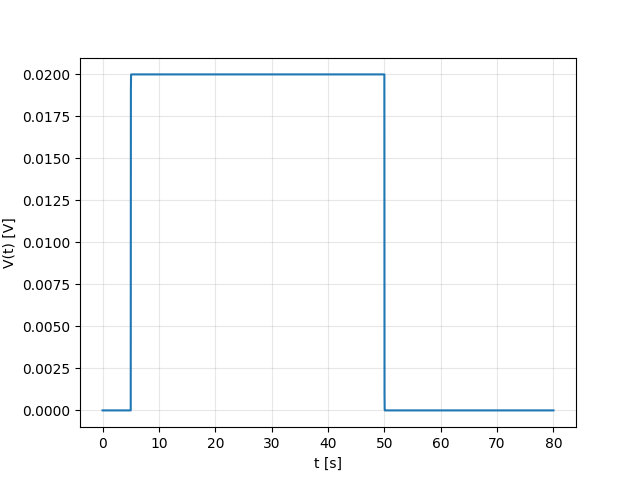
\includegraphics[width=12cm]{../ex_4.png}
		\caption{Solução por método de Euler da equação da membrana escrita no SI utiliando os valores numéricos de parâmetros da Questão 2.}
	\end{figure}
	
	Como esperado, a aparência da curva é como se, para a equação fora do SI, colocassemos valores de $g_m$ 1000 vezes maiores.\\\\
	
	\noindent\textbf{Questão 5.} Faça um estudo do efeito do tamanho do passo de iteração $\Delta t$ sobre a precisão da solução numérica fornecida pelo método de Euler em relação à solução analítica exata. Para isso, primeiramente obtenha a solução analítica da EDO da Questão 4 para o caso em que $J$ é constante desde $t=0$ e vale $2~\mu A/cm^2$. Em seguida, resolva numericamente a EDO correspondente para $0 < t < 20~ms$ com 5 valores diferentes de $\Delta t$: $\Delta t = 5 \times 10^{-4}~s$, $\Delta t = 10^{-3}~s$, $\Delta t = 2 \times 10^{-3}~s$, $\Delta t = 10^{-2}~s$ e $\Delta t = 10^{-1}~s$. Faça um gráfico de $V \times t$ com $0 < t < 20~ms$ mostrando as curvas da solução analítica e das 5 soluções numéricas obtidas, indicando cada curva por uma cor diferente. Para analisar a diferença entre uma solução numérica e a solução analítica, é conveniente calcular o erro relativo, definido como,
	\[
	ER = \frac{y_{ana} - y_{num}}{y_{ana}}.
	\]
	
	Faça outro gráfico dando os erros relativos em função de $t$, para $0 < t < 20~ms$, das soluções numéricas para os 5 diferentes valores de $\Delta t$. O que você pode concluir a respeito do efeito do tamanho do passo da iteração sobre a precisão e a estabilidade da solução numérica? Como os melhores valores de $\Delta t$ se relacionam com o valor de $\tau = R_m C_m$? Tente calcular os tempos gastos para obter as curvas numéricas para cada um dos valores de $\Delta t$ e coloque-os em uma tabela.\\\\
	
	\noindent\textbf{Resposta:} A solução analítica da equação de membrana pode ser obtida da seguinte forma:
	
	Considere a equação de membrana
	
	\begin{align*}
		\frac{dV_m(t)}{dt} = \frac{1}{C_m}\left[g_m(E - V_m(t)) + J_{\text{inj}}\right] \\
	\end{align*}
	
	que é da forma $\dot{y} = Ay + B$, para $A$ e $B$ constantes. Então, pelo método do fator integrante $u(x)$, temos
	
	\begin{align*}
		\dot{y} - Ay &= B \\
		u\dot{y} - uAy &= uB \\
	\end{align*}
	
	e, então
	
	\begin{align*}
		\dot{u} &= -Au \\
		u &= e^{-At}
	\end{align*}
	
	Assim, podemos escrever
	
	\begin{align*}
		\frac{d(ye^{-At})}{dt} &= Be^{-At}\\ 
		ye^{-At} &= B\int e^{-At} = -\frac{B}{A}e^{-At} + C \\
		y &= Ce^{At} - \frac{B}{A}				
	\end{align*}
	
	onde $C$ é uma constante definida pela condição inicial
	
	\begin{align*}
		y_0 = y(0) = C - \frac{B}{A}\\
		C = y_0 + \frac{B}{A}
	\end{align*}
	
	Finalmente,
	
	$$ y = \left(y_0 + \frac{B}{A}\right)e^{At} - \frac{B}{A}$$\\

	Considerando que $y = V_m$, $A = \frac{-g_m}{C_m}$, e $B = \frac{1}{C_m}(g_mE + J_{\text{inj}})$, temos
	
	$$V_m(t) = \left(V_0 - E - \frac{J_{\text{inj}}}{g_m}\right)e^{\frac{-g_m}{C_m}t} + \left(E + \frac{J_{\text{inj}}}{g_m}\right)$$
	\\
	
	Agora podemos plotar a solução análitica lado a lado com as soluções numéricas para cada $\Delta t$ pedido no enunciado, além de plotar o erro relativo ao longo do tempo. Veja abaixo.
	
	
	\begin{figure}[H]
		\centering
		\hspace*{-3.5cm}
		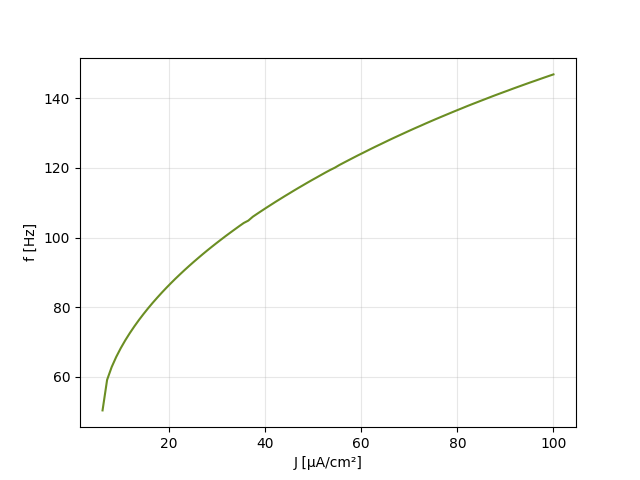
\includegraphics[width=20cm]{../ex_5.png}
		\caption{Comparação da solução analítica e das soluções numéricas para diferentes $\Delta t$ e o erro relativo.}
	\end{figure}
	
	Note que $\Delta t = 10^{-1} s = 100 ms$ é muito maior do que o domínio da solução, logo, não há como obter nenhum resultado.
	
	Com estes resultados, pode-se concluir que quanto menor o passo ($\Delta t$) utilizado na solução numérica de uma EDO, maior é a precisão e estabilidade da solução. A relação do valor de $\Delta t$ com $\tau = R_mC_m$ pode ser entendida pelo desenvolvimento abaixo. 	
	
	
	Considere a regra iterativa do método de Euler:
	
	\begin{align*}
		y(t + \Delta t) &= y(t) + y'(y(t), t)\Delta t \\
	\end{align*}
	
	Para o nosso caso, $y'(y(t), t)$ é do tipo $y' = Ay(t) + B$, onde $A$ e $B$ são constantes. Logo:
	
	\begin{align*}
		y(t + \Delta t) &= y(t) + (Ay(t) + B)\Delta t \\
		y(t + \Delta t) &= (1 + A\Delta t)y(t) + B\Delta t \\
	\end{align*}
	
	Portanto, para o passo $n$, vale:
	
	\begin{align*}
		y_n = y(t + n\Delta t) \propto (1 + A\Delta t)^n y(t)
	\end{align*}
	
	sendo o termo do lado direito a ordem mais alta em $n$. Assim, com $y(t)$ arbitrário, para que a solução não exploda para $n$ grande (o que significa $t$ grande), devemos ter a seguinte condição:
	
	\begin{align*}
		|1 + A\Delta t|^n \le 1 \\
		-1 \le 1 + A\Delta t \le 1 \\
		-2 \le A\Delta t \le 0 \\		
	\end{align*}
	
	No caso da equação de membrana, $A = \frac{-g_m}{C_m} = -\frac{1}{\tau}$. Então:
	
	\begin{align*}
		-2 \le -\frac{1}{\tau}\Delta t \le 0 \\
		2\tau \ge \Delta t \ge 0
	\end{align*}
	
	Portanto, $\Delta t \le 2\tau$ para uma solução estável da equação da membrana pelo método de Euler.
	
	O tempo para obter as curvas numéricas deste exercício foi menor do que a precisão fornecida pela minha máquina, assim, não houve diferença de tempo entre os valores de $\Delta t$: todos demoraram 0.000000...s.
	
	
	
	
	
	
	
\end{document}